\newpage
\section{Visualization}

The Orthogonal Vector Visualization System provides comprehensive visualization options for the generated vectors. This section describes the visualization techniques used by the system.

\subsection{3D Visualization}

The 3D visualization shows the vectors in three-dimensional space. It uses Matplotlib's 3D plotting capabilities to create a 3D plot with the following features:

\begin{itemize}
    \item The origin point is shown as a black dot.
    \item The vectors can be shown as arrows from the origin point or just as endpoints.
    \item Each vector is assigned a different color for easy identification, using a colormap for multiple vectors.
    \item The plot includes a legend identifying each vector.
    \item The plot includes labels for the X, Y, and Z axes.
    \item The plot includes a title, which can be customized.
\end{itemize}

The 3D visualization provides a complete view of the vectors in three-dimensional space, allowing for a better understanding of their spatial relationships.

\begin{figure}[H]
    \centering
    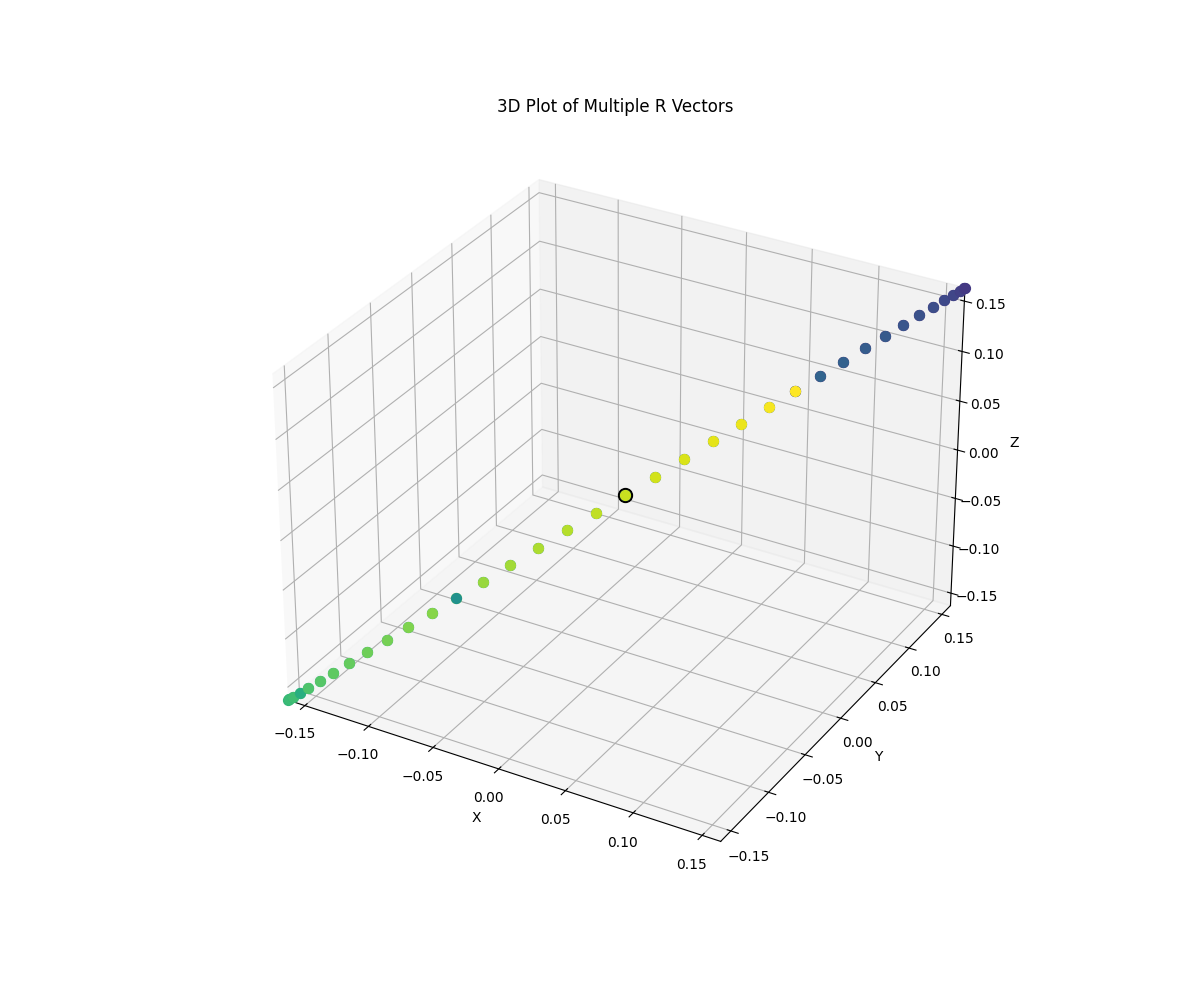
\includegraphics[width=0.8\textwidth]{figures/orthogonal_3d.png}
    \caption{Example of 3D visualization of orthogonal vectors}
    \label{fig:vis_3d_plot}
\end{figure}

\subsection{2D Projections}

The 2D visualization shows projections of the vectors onto various planes. It creates four subplots showing the following projections:

\begin{itemize}
    \item XY Plane: Shows the projection of the vectors onto the XY plane (Z=0).
    \item XZ Plane: Shows the projection of the vectors onto the XZ plane (Y=0).
    \item YZ Plane: Shows the projection of the vectors onto the YZ plane (X=0).
    \item Origin Plane: Shows the projection of the vectors onto the plane perpendicular to the vector from the global origin to the specified origin point.
\end{itemize}

Each subplot includes the following features:

\begin{itemize}
    \item The origin point is shown as a black dot.
    \item The vectors can be shown as arrows from the origin point or just as endpoints.
    \item Each vector is assigned a different color for easy identification, using a colormap for multiple vectors.
    \item The subplot includes a legend identifying each vector.
    \item The subplot includes labels for the axes.
    \item The subplot includes a title indicating the plane of projection.
\end{itemize}

The 2D projections provide different perspectives on the vectors, allowing for a better understanding of their projections onto different planes.

\begin{figure}[H]
    \centering
    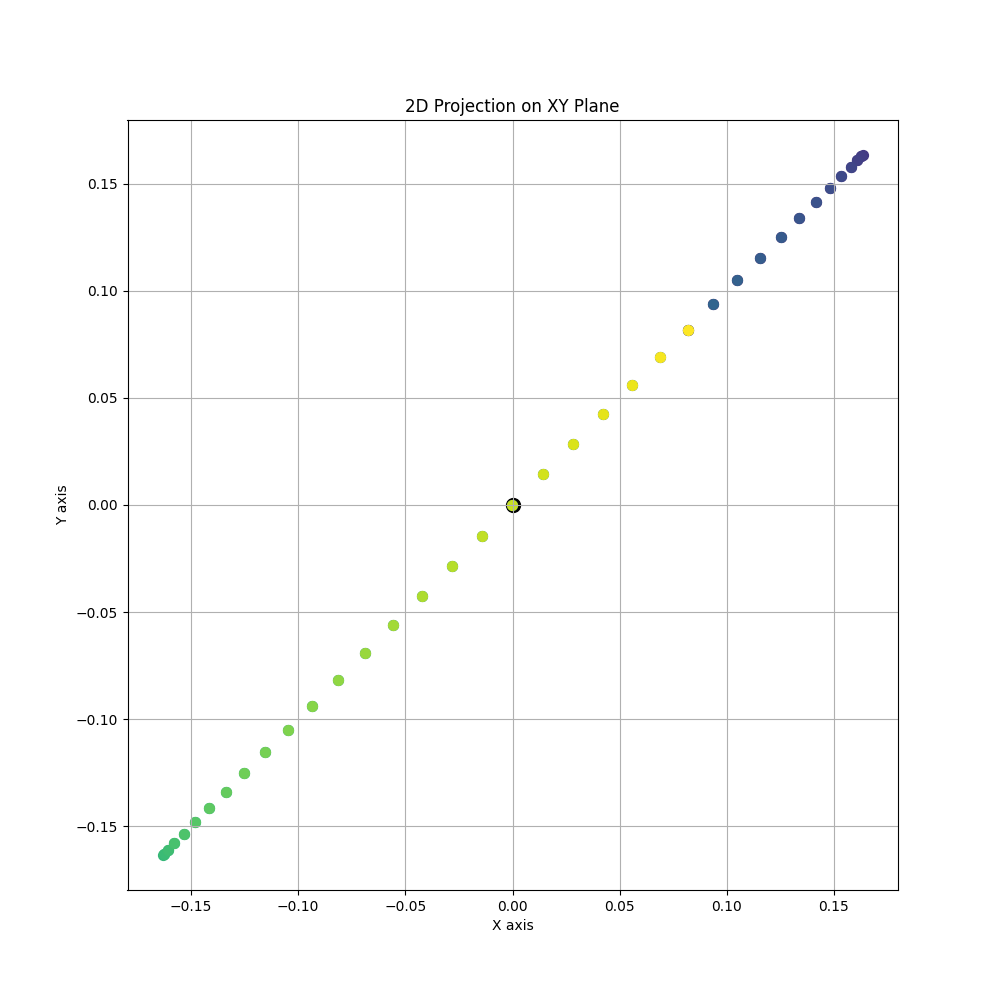
\includegraphics[width=0.45\textwidth]{figures/orthogonal_xy.png}
    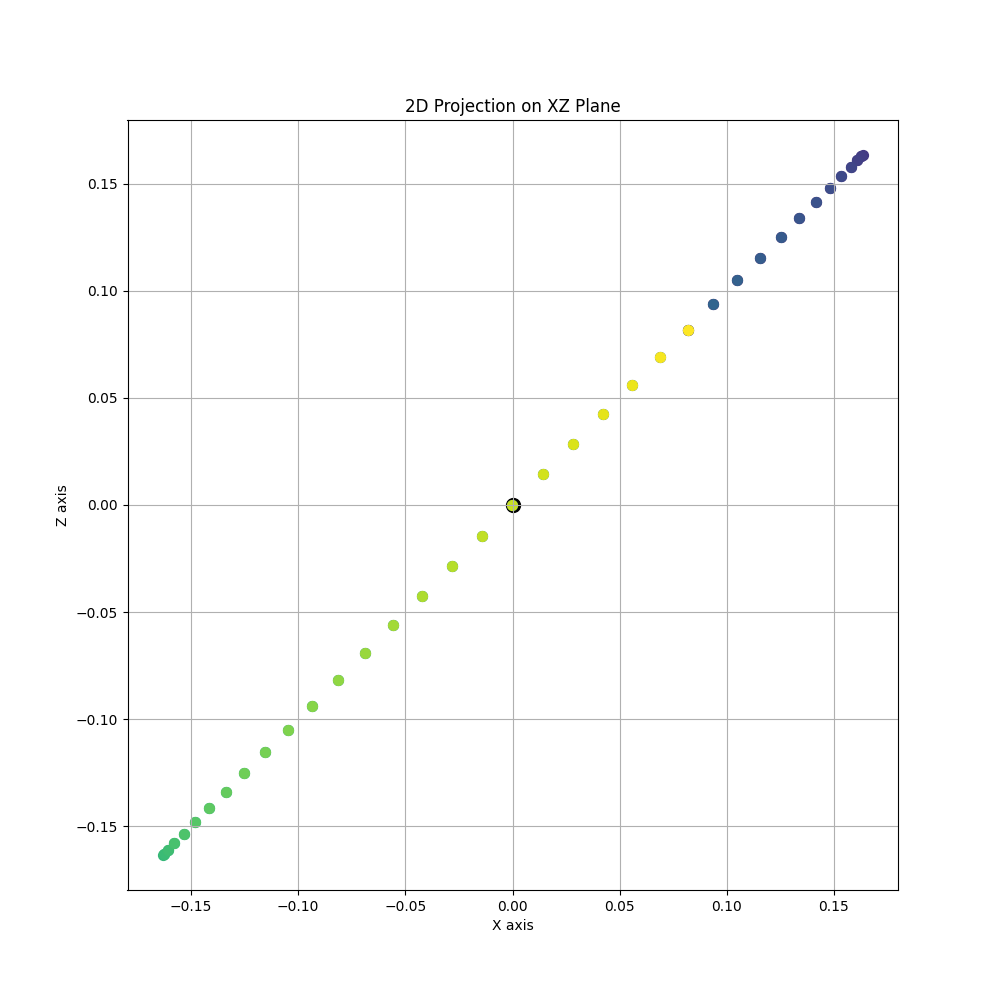
\includegraphics[width=0.45\textwidth]{figures/orthogonal_xz.png}
    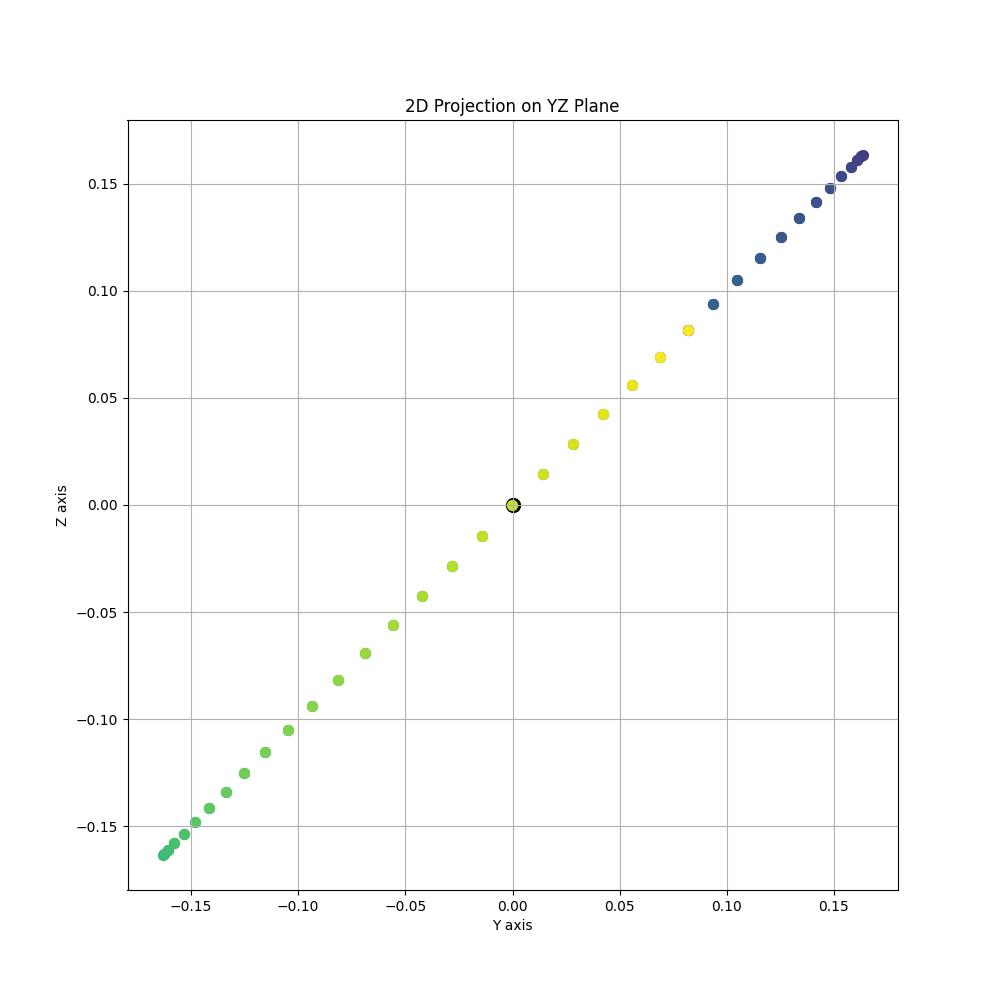
\includegraphics[width=0.45\textwidth]{figures/orthogonal_yz.png}
    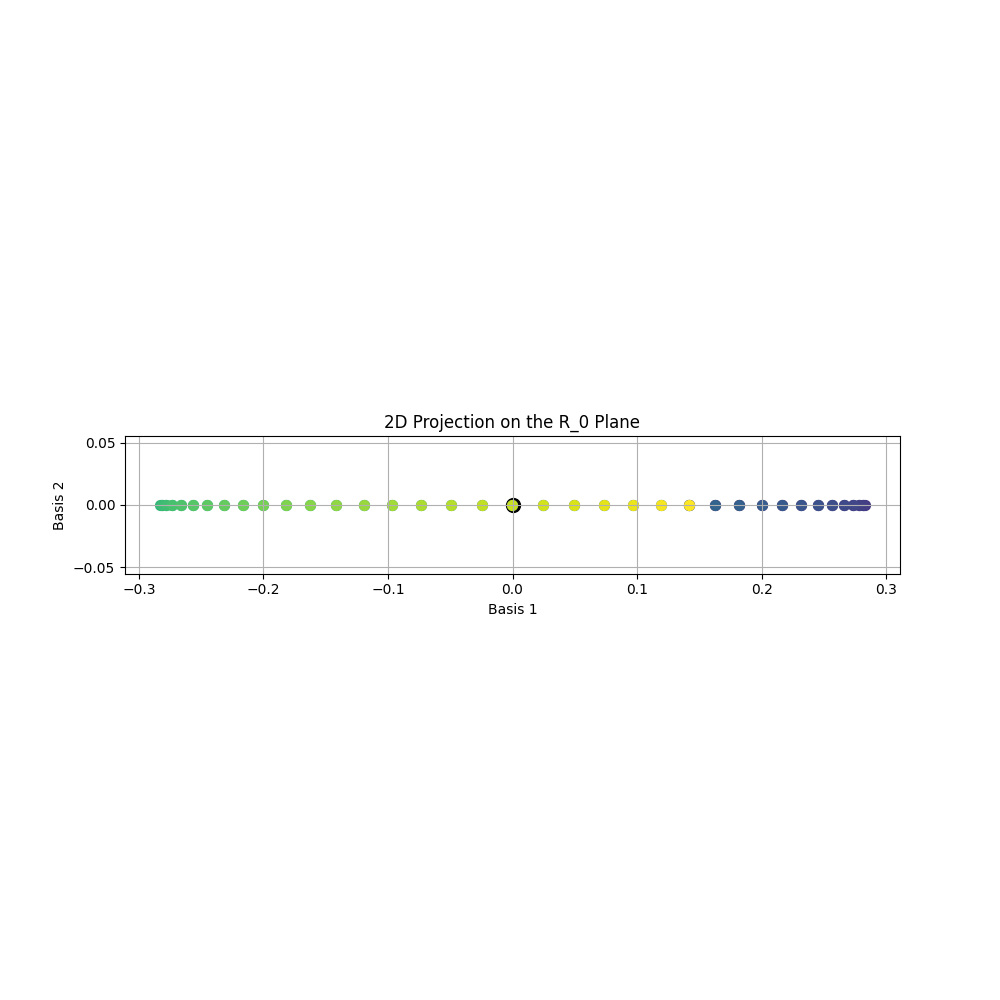
\includegraphics[width=0.45\textwidth]{figures/orthogonal_r0.png}
    \caption{Example of 2D projections of orthogonal vectors}
    \label{fig:vis_2d_projections}
\end{figure}

\subsection{Endpoints-only Plotting}

The system provides an endpoints-only plotting option that only shows the endpoints of vectors, not the arrows. This is particularly useful for visualizing patterns formed by multiple vectors, such as circle or sphere-like patterns.

\begin{itemize}
    \item In 3D visualization, the endpoints are shown as colored dots.
    \item In 2D projections, the endpoints are shown as colored dots in each projection plane.
    \item The endpoints-only option can be enabled using the --endpoints command-line option.
\end{itemize}

This option provides a clearer visualization of point patterns by removing the arrows, which can clutter the plot when there are many vectors.

\begin{figure}[H]
    \centering
    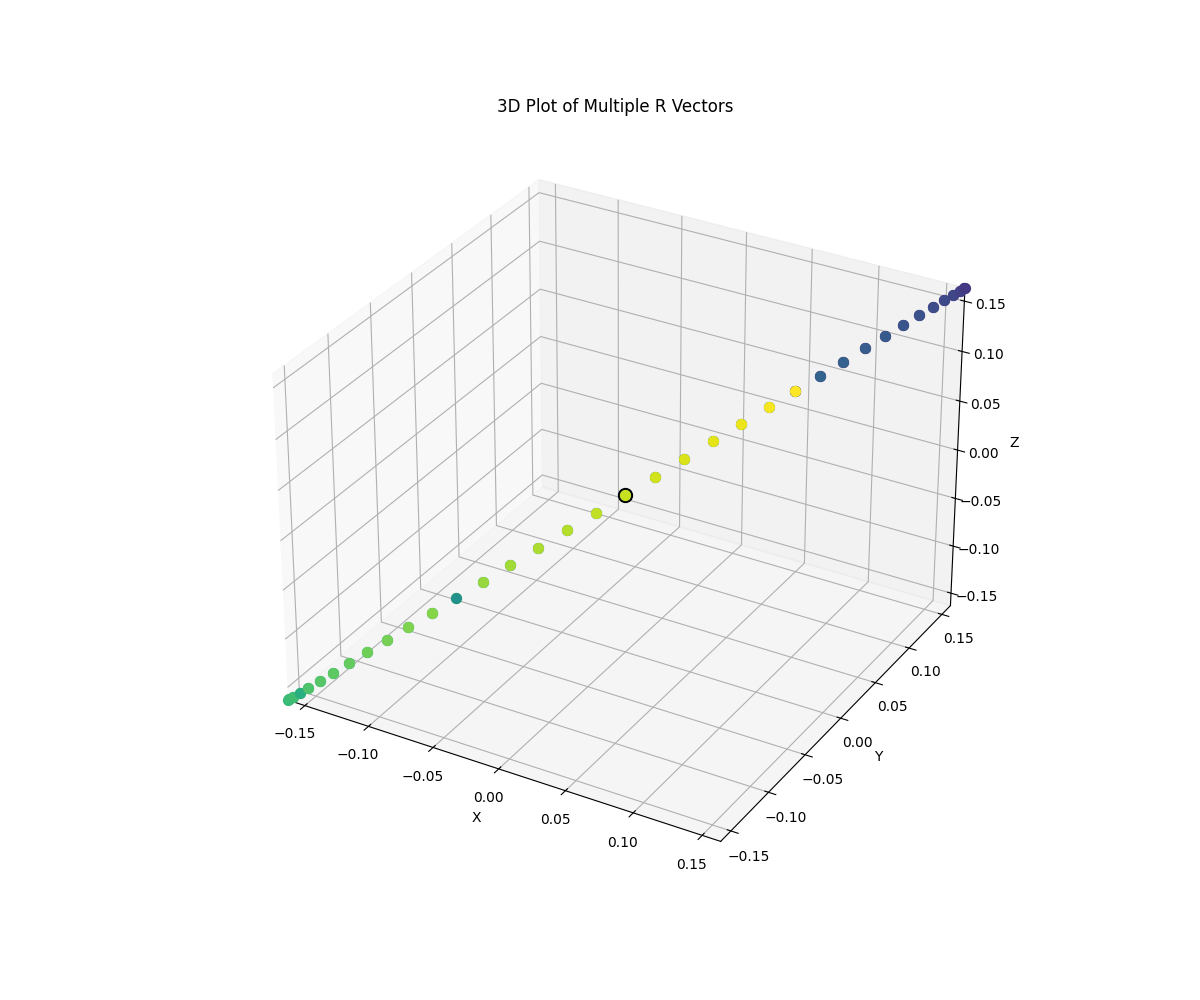
\includegraphics[width=0.8\textwidth]{figures/circle_3d.png}
    \caption{Example of endpoints-only visualization (orthogonal vector circle)}
    \label{fig:vis_endpoints_only}
\end{figure}

\subsection{Multiple Vector Visualization}

The system supports visualizing multiple vectors in a single plot, with the following features:

\begin{itemize}
    \item Multiple vectors can be generated by specifying ranges for the distance and angle parameters.
    \item Each vector is assigned a color from a colormap for easy identification.
    \item The plot includes a legend identifying each vector by its parameters.
    \item The endpoints-only option can be used to visualize the pattern formed by the endpoints of multiple vectors.
\end{itemize}

This capability is particularly useful for exploring the effects of varying parameters on the resulting vectors and for generating complex patterns such as circles and spheres.

\subsection{Circle Examples Visualization}

The system includes example scripts demonstrating different approaches to generating and visualizing circle and sphere-like patterns:

\begin{itemize}
    \item \texttt{example\_circle.py}: Generates points using orthogonal vector formulas, creating a sphere-like pattern.
    \item \texttt{example\_circle\_xy.py}: Creates a traditional circle in the XY plane.
    \item \texttt{example\_orthogonal\_circle.py}: Similar to the first example but with improved visualization.
\end{itemize}

These examples generate points at regular angular intervals and plot only the endpoints of the vectors, providing a clear visualization of the resulting patterns.

\begin{figure}[H]
    \centering
    \begin{minipage}{0.48\textwidth}
        \centering
        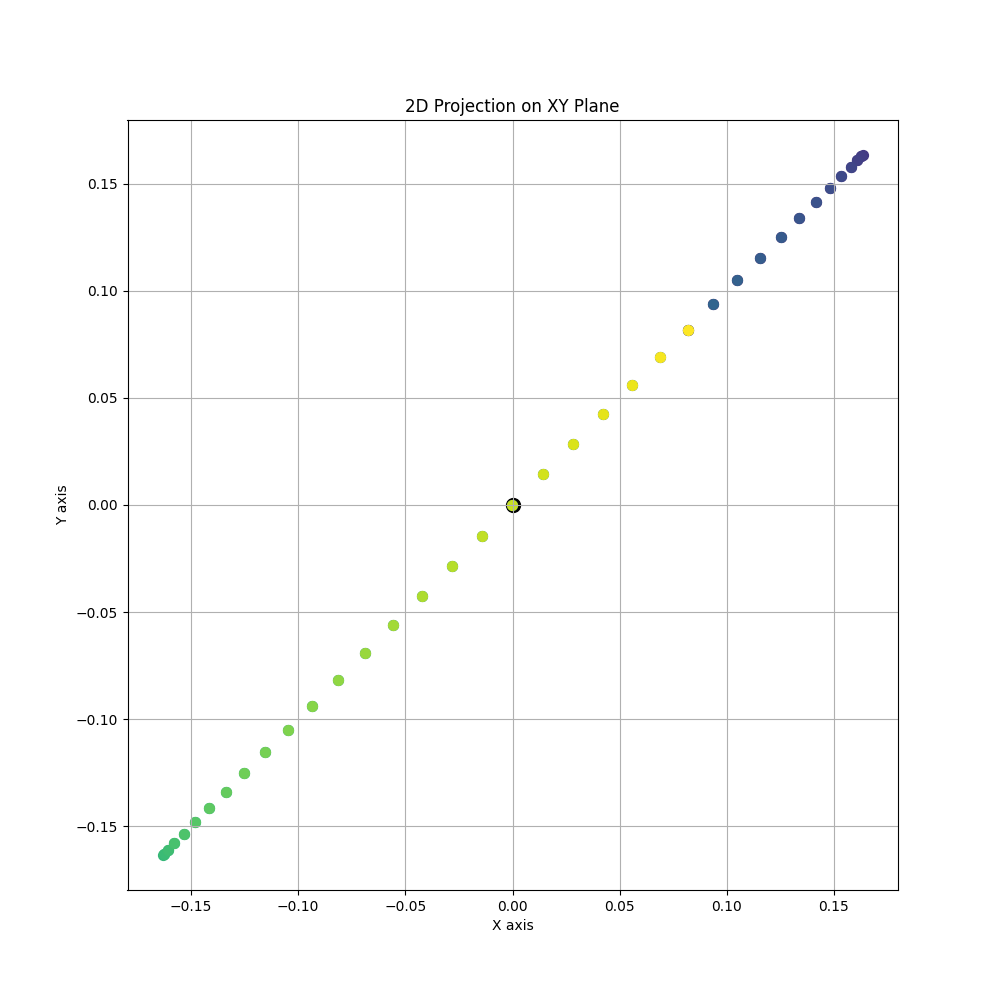
\includegraphics[width=\textwidth]{figures/circle_xy.png}
        \caption{XY projection of orthogonal vector circle}
        \label{fig:vis_circle_xy}
    \end{minipage}\hfill
    \begin{minipage}{0.48\textwidth}
        \centering
        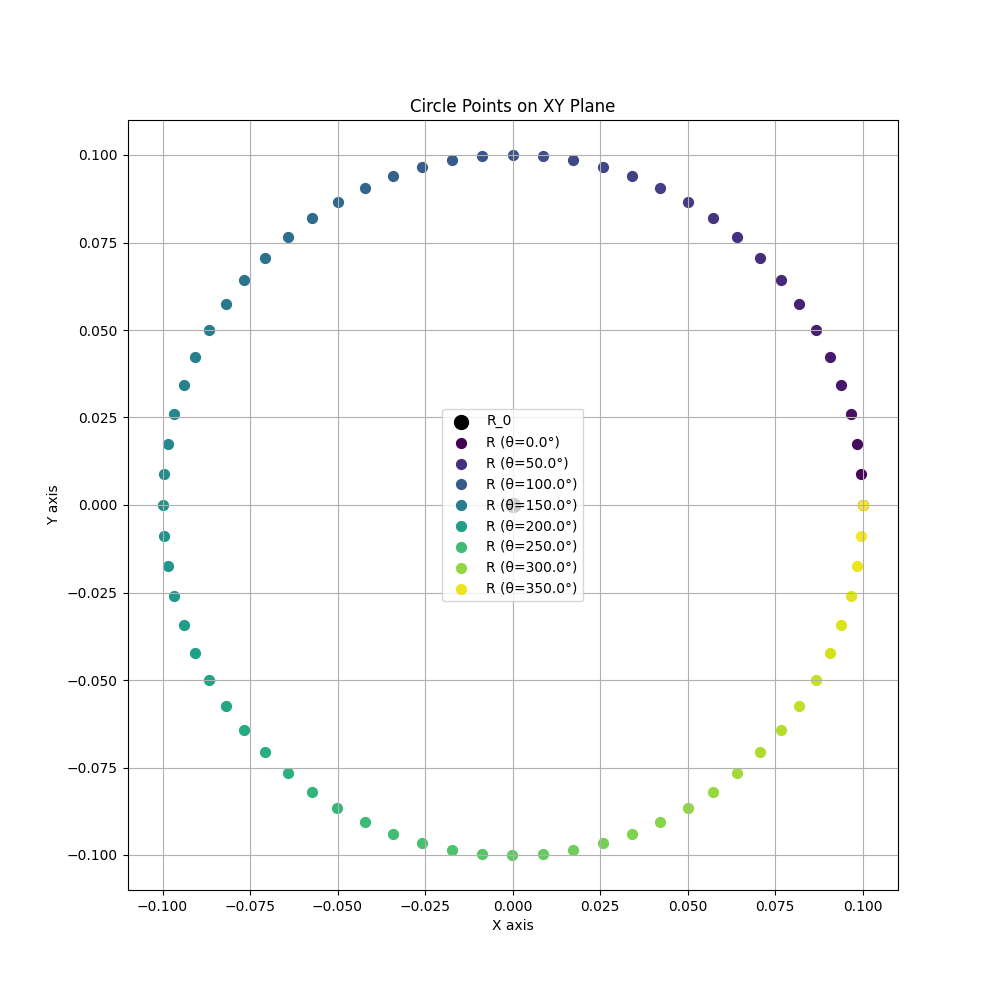
\includegraphics[width=\textwidth]{figures/xy_circle.png}
        \caption{Traditional circle in XY plane}
        \label{fig:vis_xy_circle}
    \end{minipage}
\end{figure}

\begin{figure}[H]
    \centering
    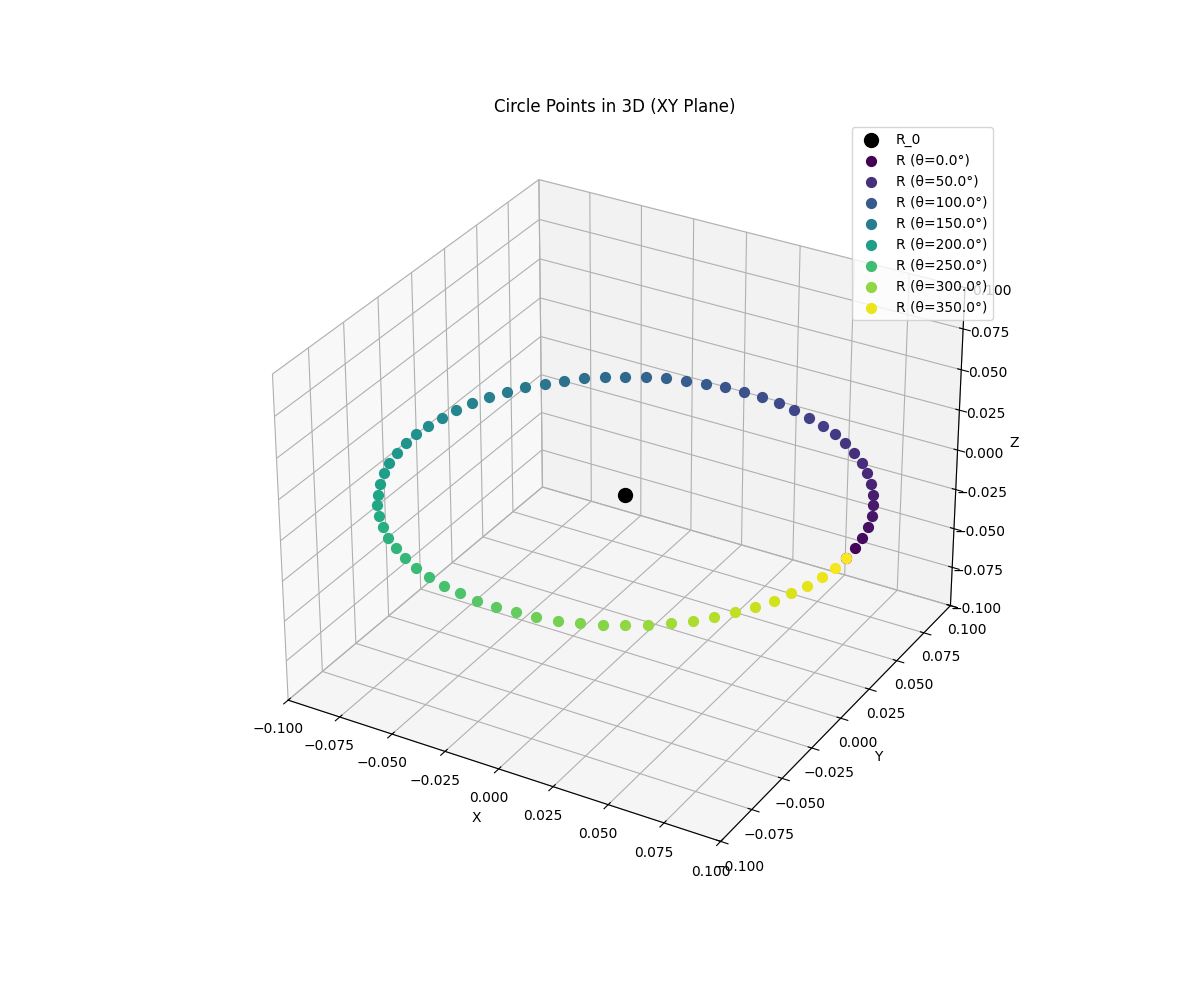
\includegraphics[width=0.8\textwidth]{figures/3d_xy_circle.png}
    \caption{3D visualization of traditional XY circle}
    \label{fig:vis_3d_xy_circle}
\end{figure}

\subsection{Implementation Details}

The visualization functions use Matplotlib to create the plots. The 3D visualization uses Matplotlib's \texttt{Axes3D} class, while the 2D visualizations use regular Matplotlib axes.

The vectors are plotted using Matplotlib's \texttt{quiver} function, which creates arrows from a starting point to an ending point. The origin point is plotted using Matplotlib's \texttt{scatter} function.

The colors of the vectors are assigned using Matplotlib's default color cycle, ensuring that each vector has a different color.

The legends are created using Matplotlib's \texttt{legend} function, with labels for each vector.

The plots are saved using Matplotlib's \texttt{savefig} function, which supports various file formats, including PNG, JPEG, and PDF.

\subsection{Visualization in the Command-line Interface}

The command-line interface provides options for controlling the visualization, including:

\begin{itemize}
    \item \texttt{--plot-type}: Specifies the type of plot, either "3d" or "2d".
    \item \texttt{--title}: Specifies the title of the plot.
    \item \texttt{--no-show}: Prevents the plot from being displayed interactively.
    \item \texttt{--save-path}: Specifies the path to save the plot.
\end{itemize}

These options allow users to customize the visualization without modifying the code.
